\documentclass[12pt]{article}
\usepackage{amssymb,amsmath,amsthm,amsfonts,mathrsfs}
\usepackage{enumitem}
\usepackage[margin=2cm]{geometry}
\usepackage{graphicx}
\usepackage[dvipsnames]{xcolor}
\usepackage{listings}
\usepackage[noend]{algpseudocode}
\usepackage{comment}
\usepackage{hyperref}
\hypersetup{
    colorlinks=true,
    linkcolor=blue,
    filecolor=magenta,
    urlcolor=blue,
    pdftitle={Overleaf Example},
    pdfpagemode=FullScreen,
    }

\title{CSC111 Project: Simulation and Map Visualization of COVID-19 Spreading Affected By Various Disease Control Policies}
\author{Marshal Guo, Yibin Cui, Zherui Zhang}
\date{April 2023}

\begin{document}

\maketitle
\section{Introduction}
Disclaimer: This project is not against any particular method or policy implemented by any world government. We respect and don't discriminate against any different undertaking that each governing body opted to do so because we must acknowledge there's no one solution that fits all situations.\\\\
With the COVID-19 pandemic drawing nearly to an end, it's an opportunity to reflect on the event and learn how to deal with an epidemic on a global scale to better prepare us for the future. \textbf{The main goal is to study how some parameters would affect the spread of COVID-19 in the selected states in the United States.} These parameters include lockdown, isolation strictness, vaccination rate, and mask-wearing mandate in a state.\\\\
We use \href{https://www.maa.org/press/periodicals/loci/joma/the-sir-model-for-spread-of-disease-the-differential-equation-model}{SIR Model} (David \& Lang) as the model for simulation of the spread of COVID-19, under the assumption that the population stays constant due to the short in nature of the disease. Then the parameters will affect the contact rate, and recovery rate, that are involved in the SIR Model.
\newpage
\section{Datasets}
Datasets were a crucial part of our project. First, we found a dataset "states.csv" (Rozanec) that contains each state's name and its latitude and longitude. We then merged it with another dataset "State Populations.csv" (Gill) that contains the population of each state as the following. With this dataset, we are able to initialize the beginning phase of the program by populating and locating each State object. The coordinates also contribute to the infect\_next\_state() algorithm that will be addressed in the computational section of this report. We also made smaller versions of this dataset by either reducing the population in each state or number of states or both just to reduce the computation and running time for testing and presentation purposes.

\begin{center}
\begin{tabular}{|c c c c|}
 \hline
 State & Latitude & Longitude & Population \\ [0.5ex]
 \hline\hline
 Alabama & 32.7794 & -86.8287 & 4888949 \\
 \hline
 Alaska & 64.0685 & -152.2782 & 738068 \\
 \hline
 Arizona & 34.2744 & -111.6602 & 7123898 \\
 \hline
 ... & ... & ... & ... \\
\end{tabular}
\end{center}
At the end stages of the simulation, we export a dataset to make it convenient for Plotly to plot the map onto the webpage. The written CSV file consists of information on the starting latitude and longitude of the starting state and the ending latitude and longitude of the receiving state. The format is as follows.

\begin{center}
\begin{tabular}{|c c c c c c|}
 \hline
 start\_lat & start\_lon & end\_lat & end\_lon & state1 & state2 \\ [0.5ex]
 \hline\hline
 64.0685 & -152.2782& 34.2744& -111.6602 & Alaska & Arizona\\
 \hline
 ... & ... & ... & ... & ... & ... \\
\end{tabular}
\end{center}
To reduce the confusion you may encounter in understanding each csv files, I will list the names and functions of all the csv files used in this project. In the data zip file we uploaded on MarkUs, there are five csv files, which are state\_full.csv, state\_several.csv, state\_small.csv, state\_many.csv, and state\_full\_population\_not\_full. The state\_full.csv contains all U.S. states as well as the true state populations for 2018, which were obtained by fusing the two reference files mentioned above. For the rest of the four csv files, each file contains a different number of states, which you can easily identify by their names. In addition, the number of people in each state has been significantly reduced in order to increase the efficiency of the computer. Also, the csv file we generated is named edges.csv, and it is not in the data folder, instead, it's in the 'main' folder.

\newpage
\section{Computational Overview}
We use graph to simulate the spread of the virus between the selected states, in the file `graph.py'.\\\\
\textbf{sir\_model.py}\\
There are `Susceptible', `Infective', and `Removal' datatype to represent the three groups of people in the SIR Model (David \& Lang), while each person is represented by a `Person' class, that has a unique id. In the `Susceptible', 'Infective', and `Removal' datatype, there are methods for adding and removing people from each type, that will be used for simulation during the spread of COVID-19.\\\\
\textbf{graph.py} \\
We use the `State' class for representing each state selected, with attributes `sus', `inf', `rem' representing the three groups in the SIR Model (David \& Lang), and a and r for representing the rate of removal and rate of contact, and other attributes are as described as in the file.\\
And the `InfectedZones' class is a graph for representing the infected states among selected states in US. It will be initialized with all selected states, its methods are used during the simulation.\\
The `infection\_process' method of `State' is the method for simulating the infection from the certain state, it updates the spread within the state everyday by the following algorithm.\\
\newcommand{\n}{\hspace*{5mm}}
\n \textbf{Algorithm (Tom)}.\\
\n We use day to be unit of time.\\
\n Let $S$ denote the number of people in sus, $S_0$ be the initial value of $S$.\\
\n Let $I$ denote the number of people in inf, $I_0$ be the initial value of $I$.\\
\n Let $R$ denote the number of people in rem, $R_0$ be the initial value of $R$.\\
\n By our assumption that there is no birth, the sum $S+I+R$ is constant over the \\\n time.\\
\n And we need to update the three values each day using $r$, which is the infection rate, and $a$, \\\n which is the recovery rate.\\
\n There is a difference in the algorithm comparing to the standard SIR Model (David \& Lang), \n that is, a person is able to recover only if the person has been infected more than $14$ days.\\
\n Therefore let $I'$ denote the number of people in inf that has been infected more than $14$ days.\\
\n Then we have
\[\frac{dS}{dT} = -rIS\]
\[\frac{dI}{dS} = rIS-aI'\]
\[\frac{dR}{dT} = aI'\]
\n In each day during the infection process, the method first remove $rIS$ people from the state's \\\n `sus', and set these people to the state's `inf', then remove $aI'$ people from the state's `inf', and \\\n set these people to the state's `rem'.\\\\
Then it will try to infect another state, using the method `infect\_next\_state'. The `infect\_next\_state' method's algorithm is as described in its docstring in the file.\\
The infection process will finish when there are no infective people.\\
The InfectedZones method `add\_state' will get the given state infected, randomly choose a patient zero for the State object using the `get\_patient\_zero' method, then starts the infection process using the `infection\_process' method.\\\\
A few notes:
\begin{enumerate}[label = \roman*.]
    \item A state can infect other states only if there are more than `TRANSMIT\_THRESHOLD' (a provided constant) infective people.
    \item A state that is under lockdown is harder to infect another state.
    \item For every infected people, their infected days are also increased by one in each day of the infection process.
    \item The method `infection\_process' uses a recursion, although not directly represented in the implementation. But notice that when infecting next state, the State method `infect\_next\_state' is called, in which the InfectedZones method `add\_state' is called to modify the InfectedZones object, in which `infect\_next\_state' is called again.
\end{enumerate}$\\$
\textbf{simulation.py}\\
The function `populate\_states' reads a csv file under the `data' folder, and return a tuple containing a dictionary mapping every state's name to a created State object representing the state, and a list of states' names. Note that when creating the State object, \textbf{all} people in the state is set in `sus' attribute, which means all people are considered to be susceptible at the beginning.\\
The function `graph\_to\_csv' takes an InfectedZone as the input, and create a new csv file. The created csv file contains the two states' location (latitude and longitude), and their names. Then the file will be saved in the project folder. The file is for plotting the diagram.\\
The function `get\_user\_input' is the interactive function, for the user to choose the parameters when running the main file.\\\\
\textbf{plotter.py}\\
The Plotter module only contains the plot\_diagram() function that takes in two arguments, the path of the dataset, i.e. 'states\_small.csv', that was used to initialize the state objects and the path that contains the dataset that contains the edges info of the graph structure, namely 'edges.csv'. Given the information stored in the columns, we plot the connections between infected states using lines and locate the states using dots.
\\\\
\textbf{main.py}\\
Our main file for running the simulation.\\
The dataset can be selected from the files under the data folder. However, the `states\_full.csv' is not recommended, for two reasons. First, the population is too large, and since we represent each person with unique id, it is time-consuming to run with it. Second, the contact rate $r$ need to be modify, since the population are much larger than other example files, the contact rate will need to be lowered.\\
The function `main' will first call the `populate\_states' function to process the selected dataset file, and then initialize the InfectedZones with the data.\\
Then user is allowed to enter the paramaters for each state following the instruction, the parameters will be saved in each State object in the InfectedZones object. The instruction for the interactive part is in the next section.\\
Then a unlucky state is randomly picked to be the origin of COVID-19, and `add\_state' method is called, which would start the simulation of the infection process.\\
When the infection process finishes, the data will be saved as a new csv file using `graph\_to\_csv' function.\\
Finally, `plot\_diagram' is called to create the diagram representation of the infection process.
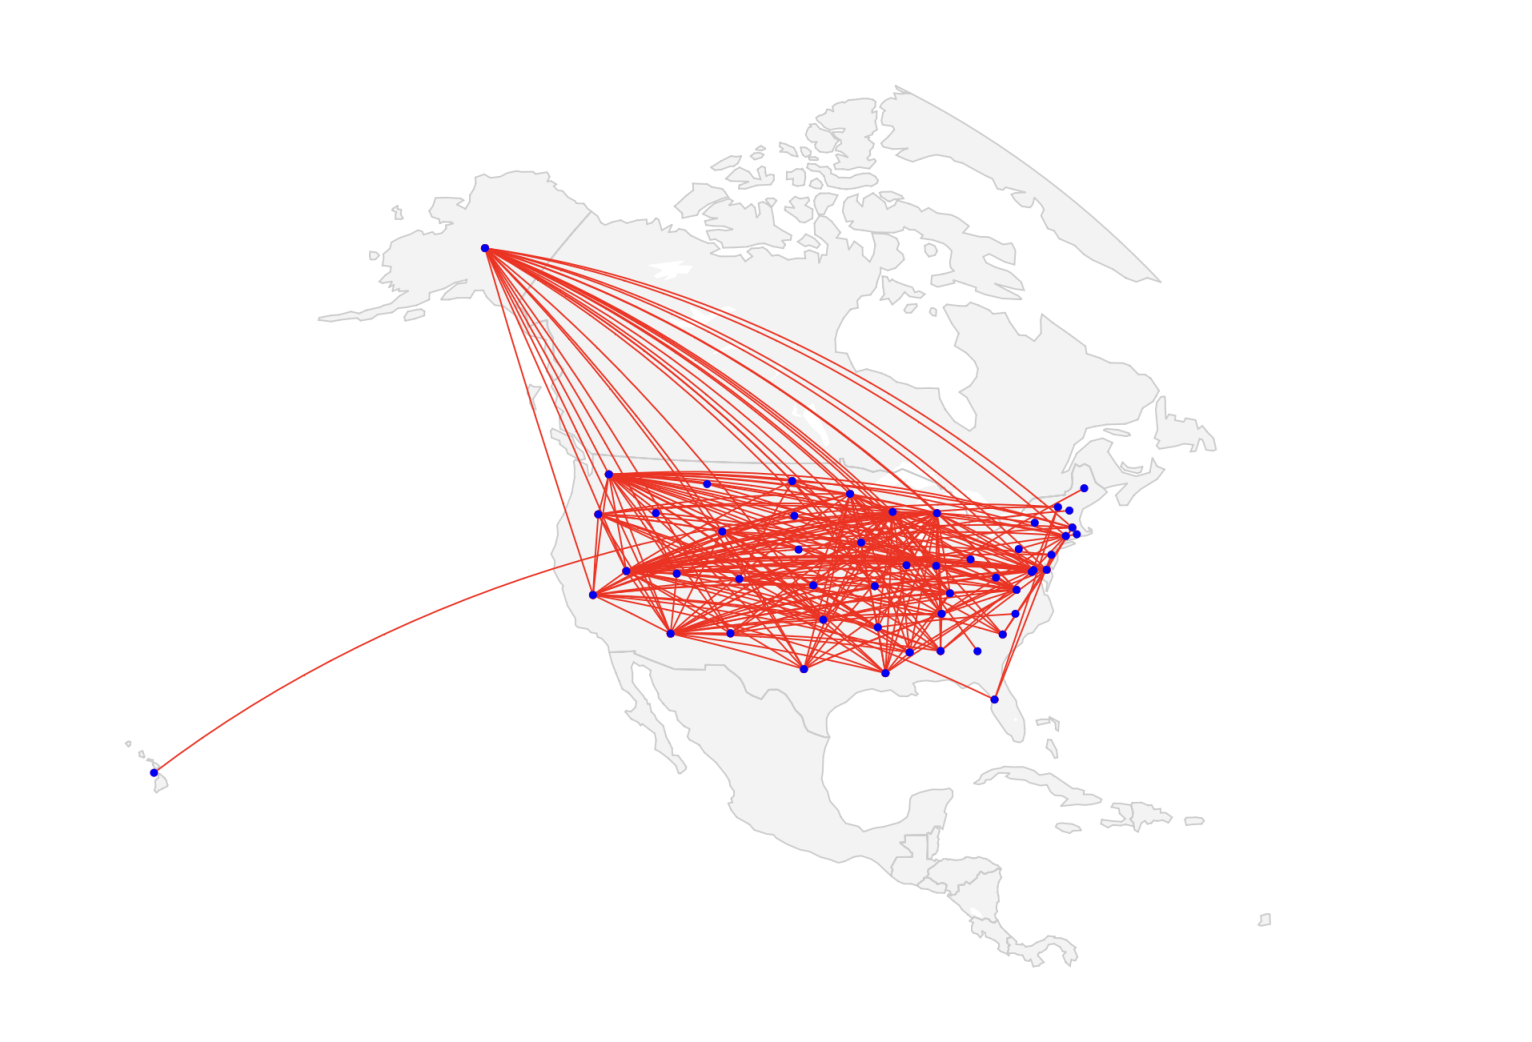
\includegraphics[scale=0.3]{project_im2.png}
$\\$This is the visual representation of the infection process, with all default parameters, with dataset is `states\_full\_people\_not\_full.csv'

\newpage
\section{Instructions for obtaining datasets and running program}
In this sections detailed instructions for obtaining datasets and running program is presented.\\\\
\textbf{Python library requirement}\\
Our project is 'pure python' we did not use other programming languages or non-python software. Therefore the python library requirement is relatively simple, we only used python-ta for checking code as well as plotly and panadas for graphics and data visualization. We provided a requirement.txt file for you to download python libraries, so feel free to use it.\\\\
\textbf{Instructions for downloading datasets}\\
For our project, we have provided the datasets for you, the zip file named data we've uploaded on MarkUs, which is under 25MB, includes all the csv files that is required to run the program. Also, if you run the program, there should be a file named edges.csv being created, this csv file is generated by a function defined by us, and this csv file is rewritten every time you run the program.\\\\
\textbf{Instructions for running program}\\
For running our program, you may open the file named main.py, we have implemented a main() function to start our COVID-19 simulation, and we have created a main block at the bottom of the file. So, when you run this file in python console, the simulation begins.
By the time python console pops up, you should see this sentence printed:\\
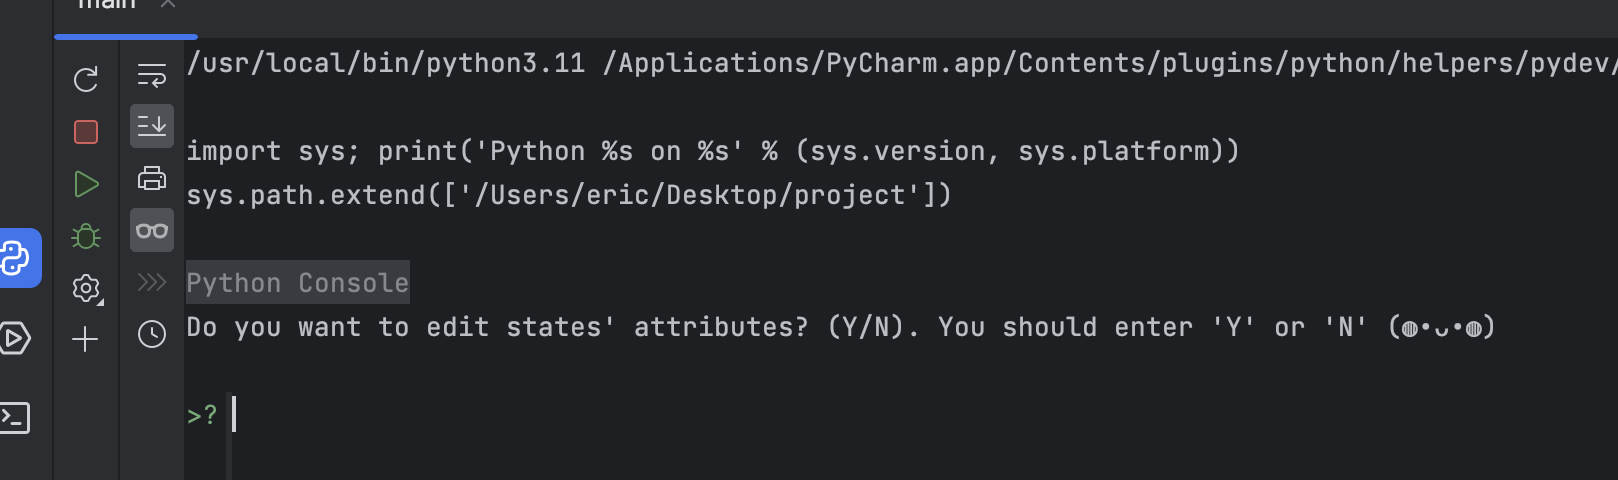
\includegraphics[scale=0.5]{image1.png}\\
For experimenting with how changing attributes of a state would affect outcomes, you may enter Y, but if you enter N or other inputs, all states' attributes will be initialized to the default value. We recommend you to enter Y only if you are experimenting with a csv file containing only few states, because it would be a bit time-consuming if you change many states' attributes. However, you are more than welcome to try if you want to.\\
Assuming you entered Y for that question, you should see these sentences printed:\\
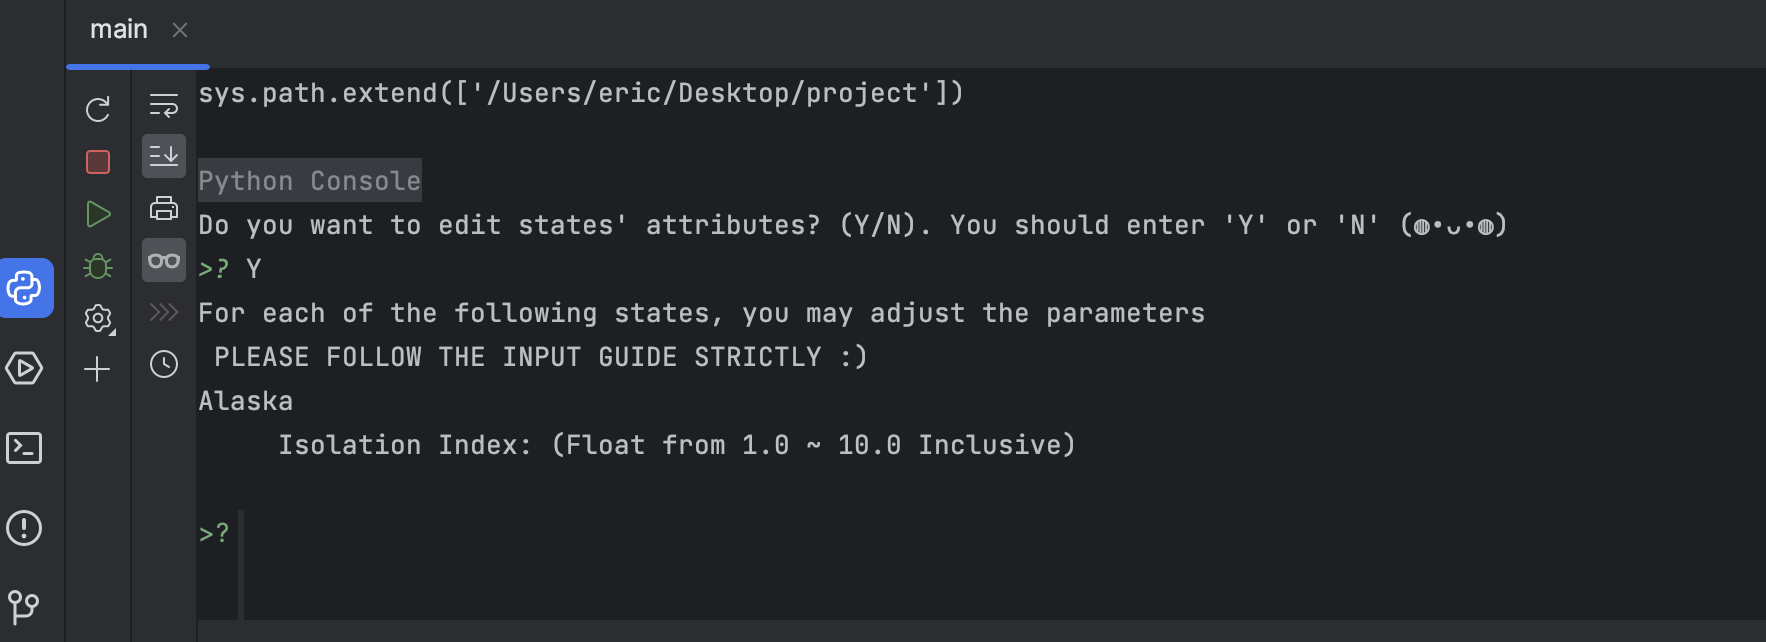
\includegraphics[scale=0.45]{image2.png}\\
Using this as an example, You are about to change the isolation attribute of a state named Alaska. By the sentence in brackets, you are encouraged to enter a float from 1.0 to 10.0, the float you enter will be state.isolation. However, if you enter a float outside the scope, this function will still proceed, because we didn't use check\_contracts. But, you may not do that since that input violates the precondition of this function, and the representation invariants of the State class.\\
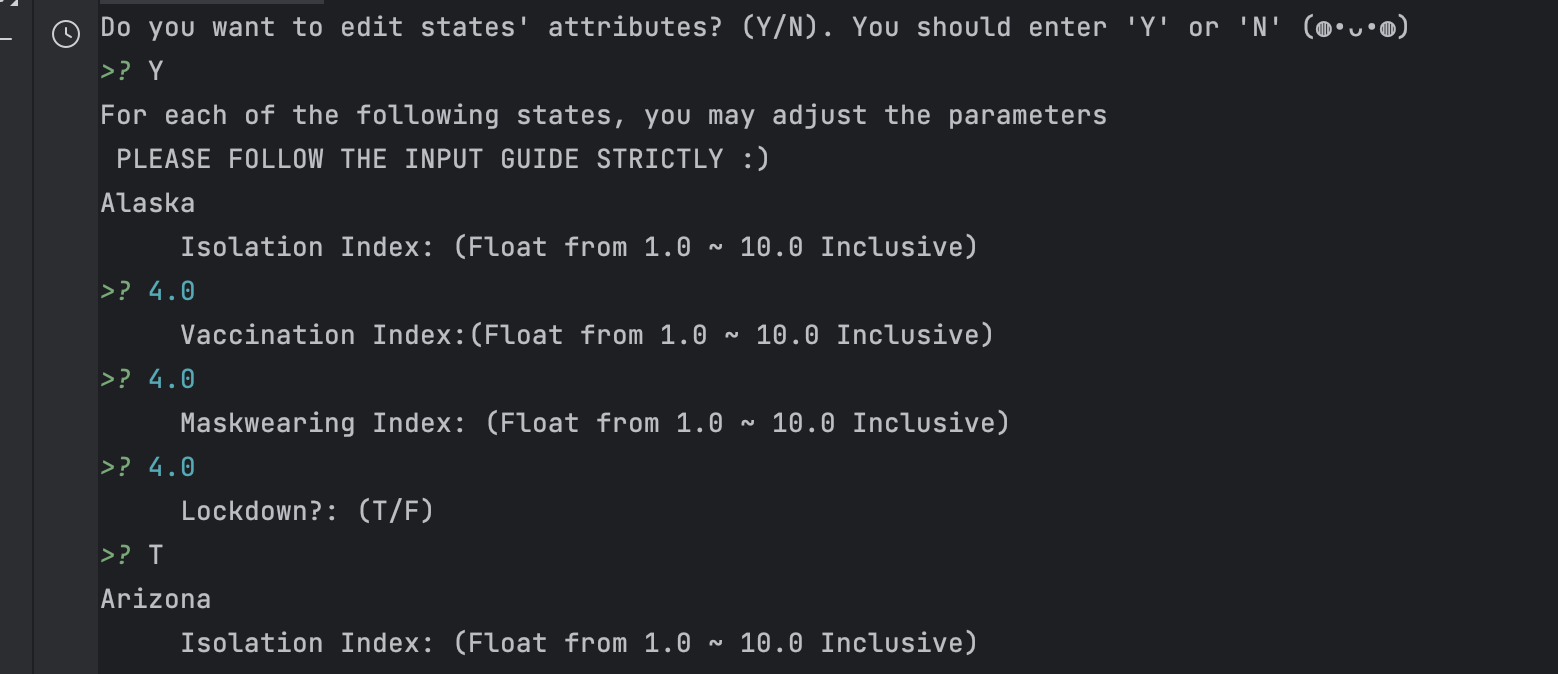
\includegraphics[scale=0.5]{image3.png}\\
The image above provides an example of how you may respond to each question. After setting the four attributes, the function iterates and you are able to change next state's attribute question. After you finish modifying all states' attributes the function will proceed. Worth mentioning that for answering lockdown attributes, it is only set True if you enter T, if you enter F or other input, it will be set to False. Note that all of these attributes will have an impact on the outcome of the simulation, you may refer to the algorithm section above or the functions docstrings in each python file we submitted to understand how the algorithm works. Additionally, you may change the value of rate of removal and rate of contact in simulations.py and transmit\_threshold in graph.py for further experiments but it is completely optional, since we have already set a reasonable default value.
Assuming the function proceeds, next comes calculating infection and recovery people within states, as well as spread of disease across states. You may refer to graph.py and sir\_model.py for more precise information. The python console will print out a lot of data while this process is going on. You may feel that the data is a bit messy, but this is due to the fact that we are using recursion function calls, and our function runs without problems. If you do not want to see the data printed, you may go to graph.py, under the State class there is a infection process function, in this function you may comment out or delete print() calls.\\
As people in all states recover, the final phase of the simulation begins. Our function creates a csv file based on the simulation outcome. Next, by automatically triggering the function that draws the graph in plotter.py, the direct disease transmission routes between each state with other states is drawn, you will see the visualization of the graph in a pop-up page.\\
It is important to note that due to the random nature of the spread of the epidemic, it is normal that the map is drawn differently each time you run the simulation, namely the connection between states is different. Each state is marked with a blue dot and the name of the corresponding state is automatically displayed when your cursor touch a blue dot. The transmission paths are all connected by red lines, which is obvious.\\
Finally, you are more than welcome to change DATASET = '....csv' in main.py, note that the csv file should be a file in the data folder, which is obtained by unzipping data.zip that we submitted on MarkUs. Also, you can freely change values in each csv file that is in the data folder. However, we do not recommend you to set DATASET = 'data/state\_full.csv' since it is created using actual data, so it is very time-consuming to run. \\I will paste a few images of the final results below for reference only.\\
Example graph of mutual contagion among the states:\\
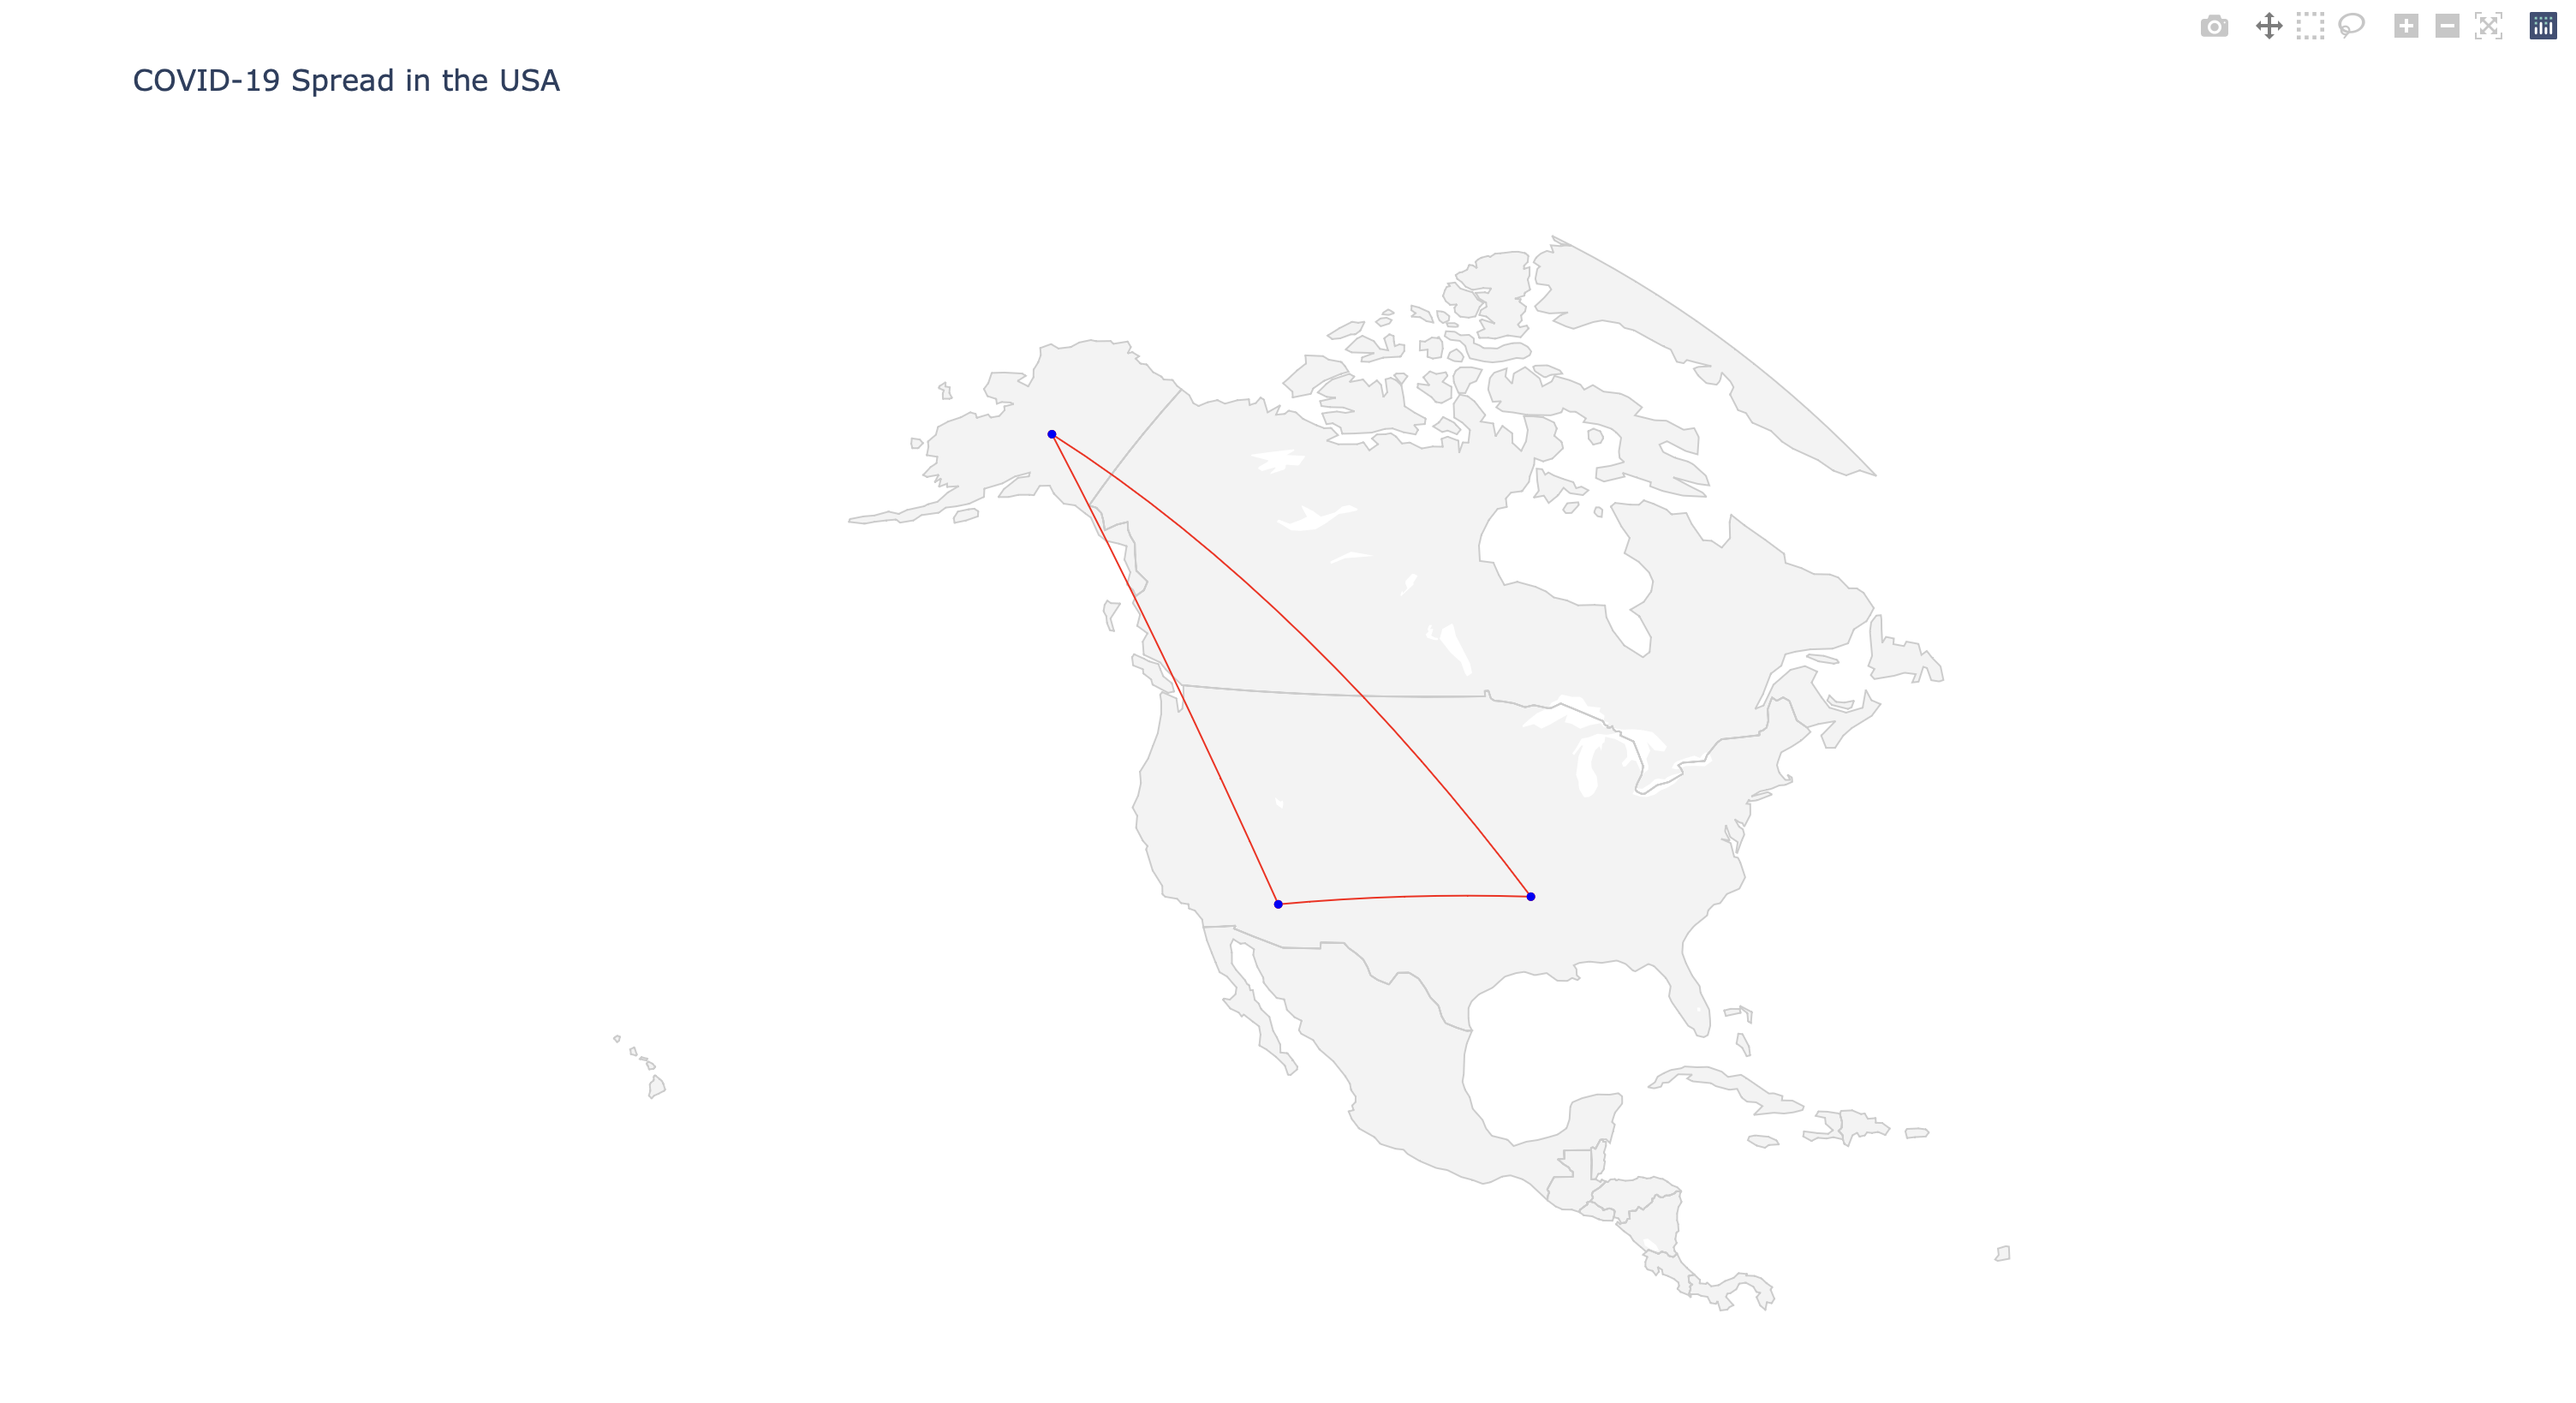
\includegraphics[scale=0.25]{image4.png}\\
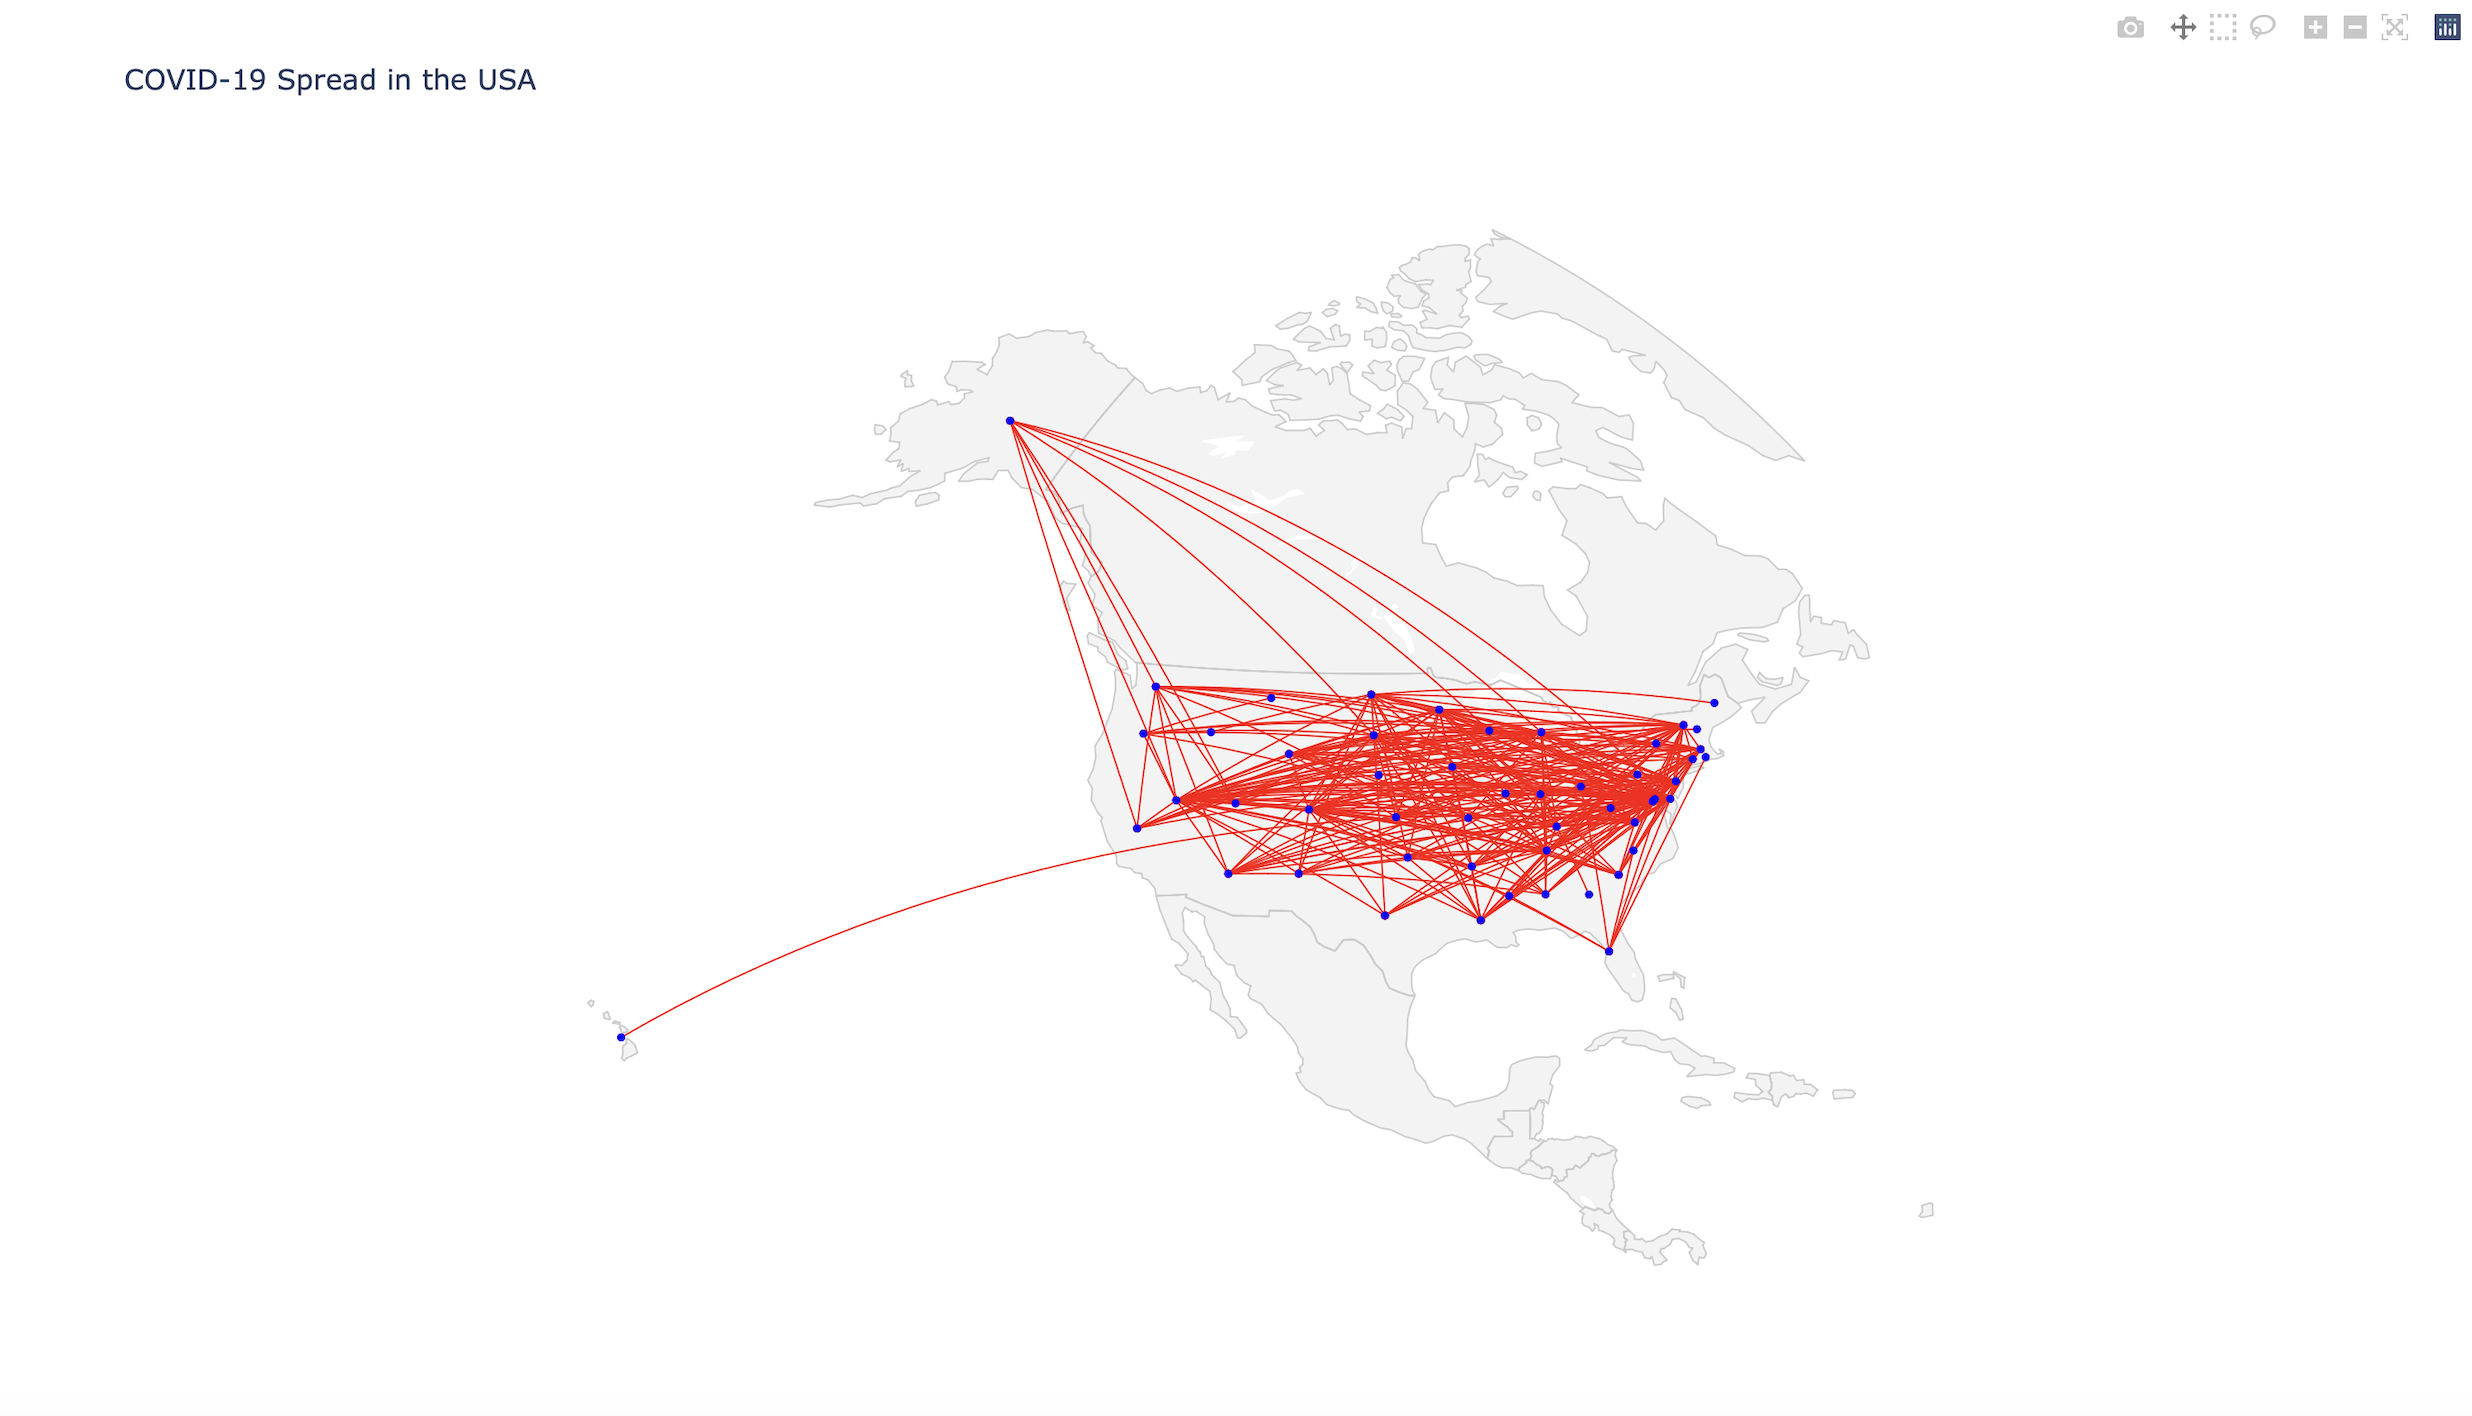
\includegraphics[scale=0.3]{image6.png}\\
Example graph of no cross-transmission of viruses between each state (change state's attributes):\\
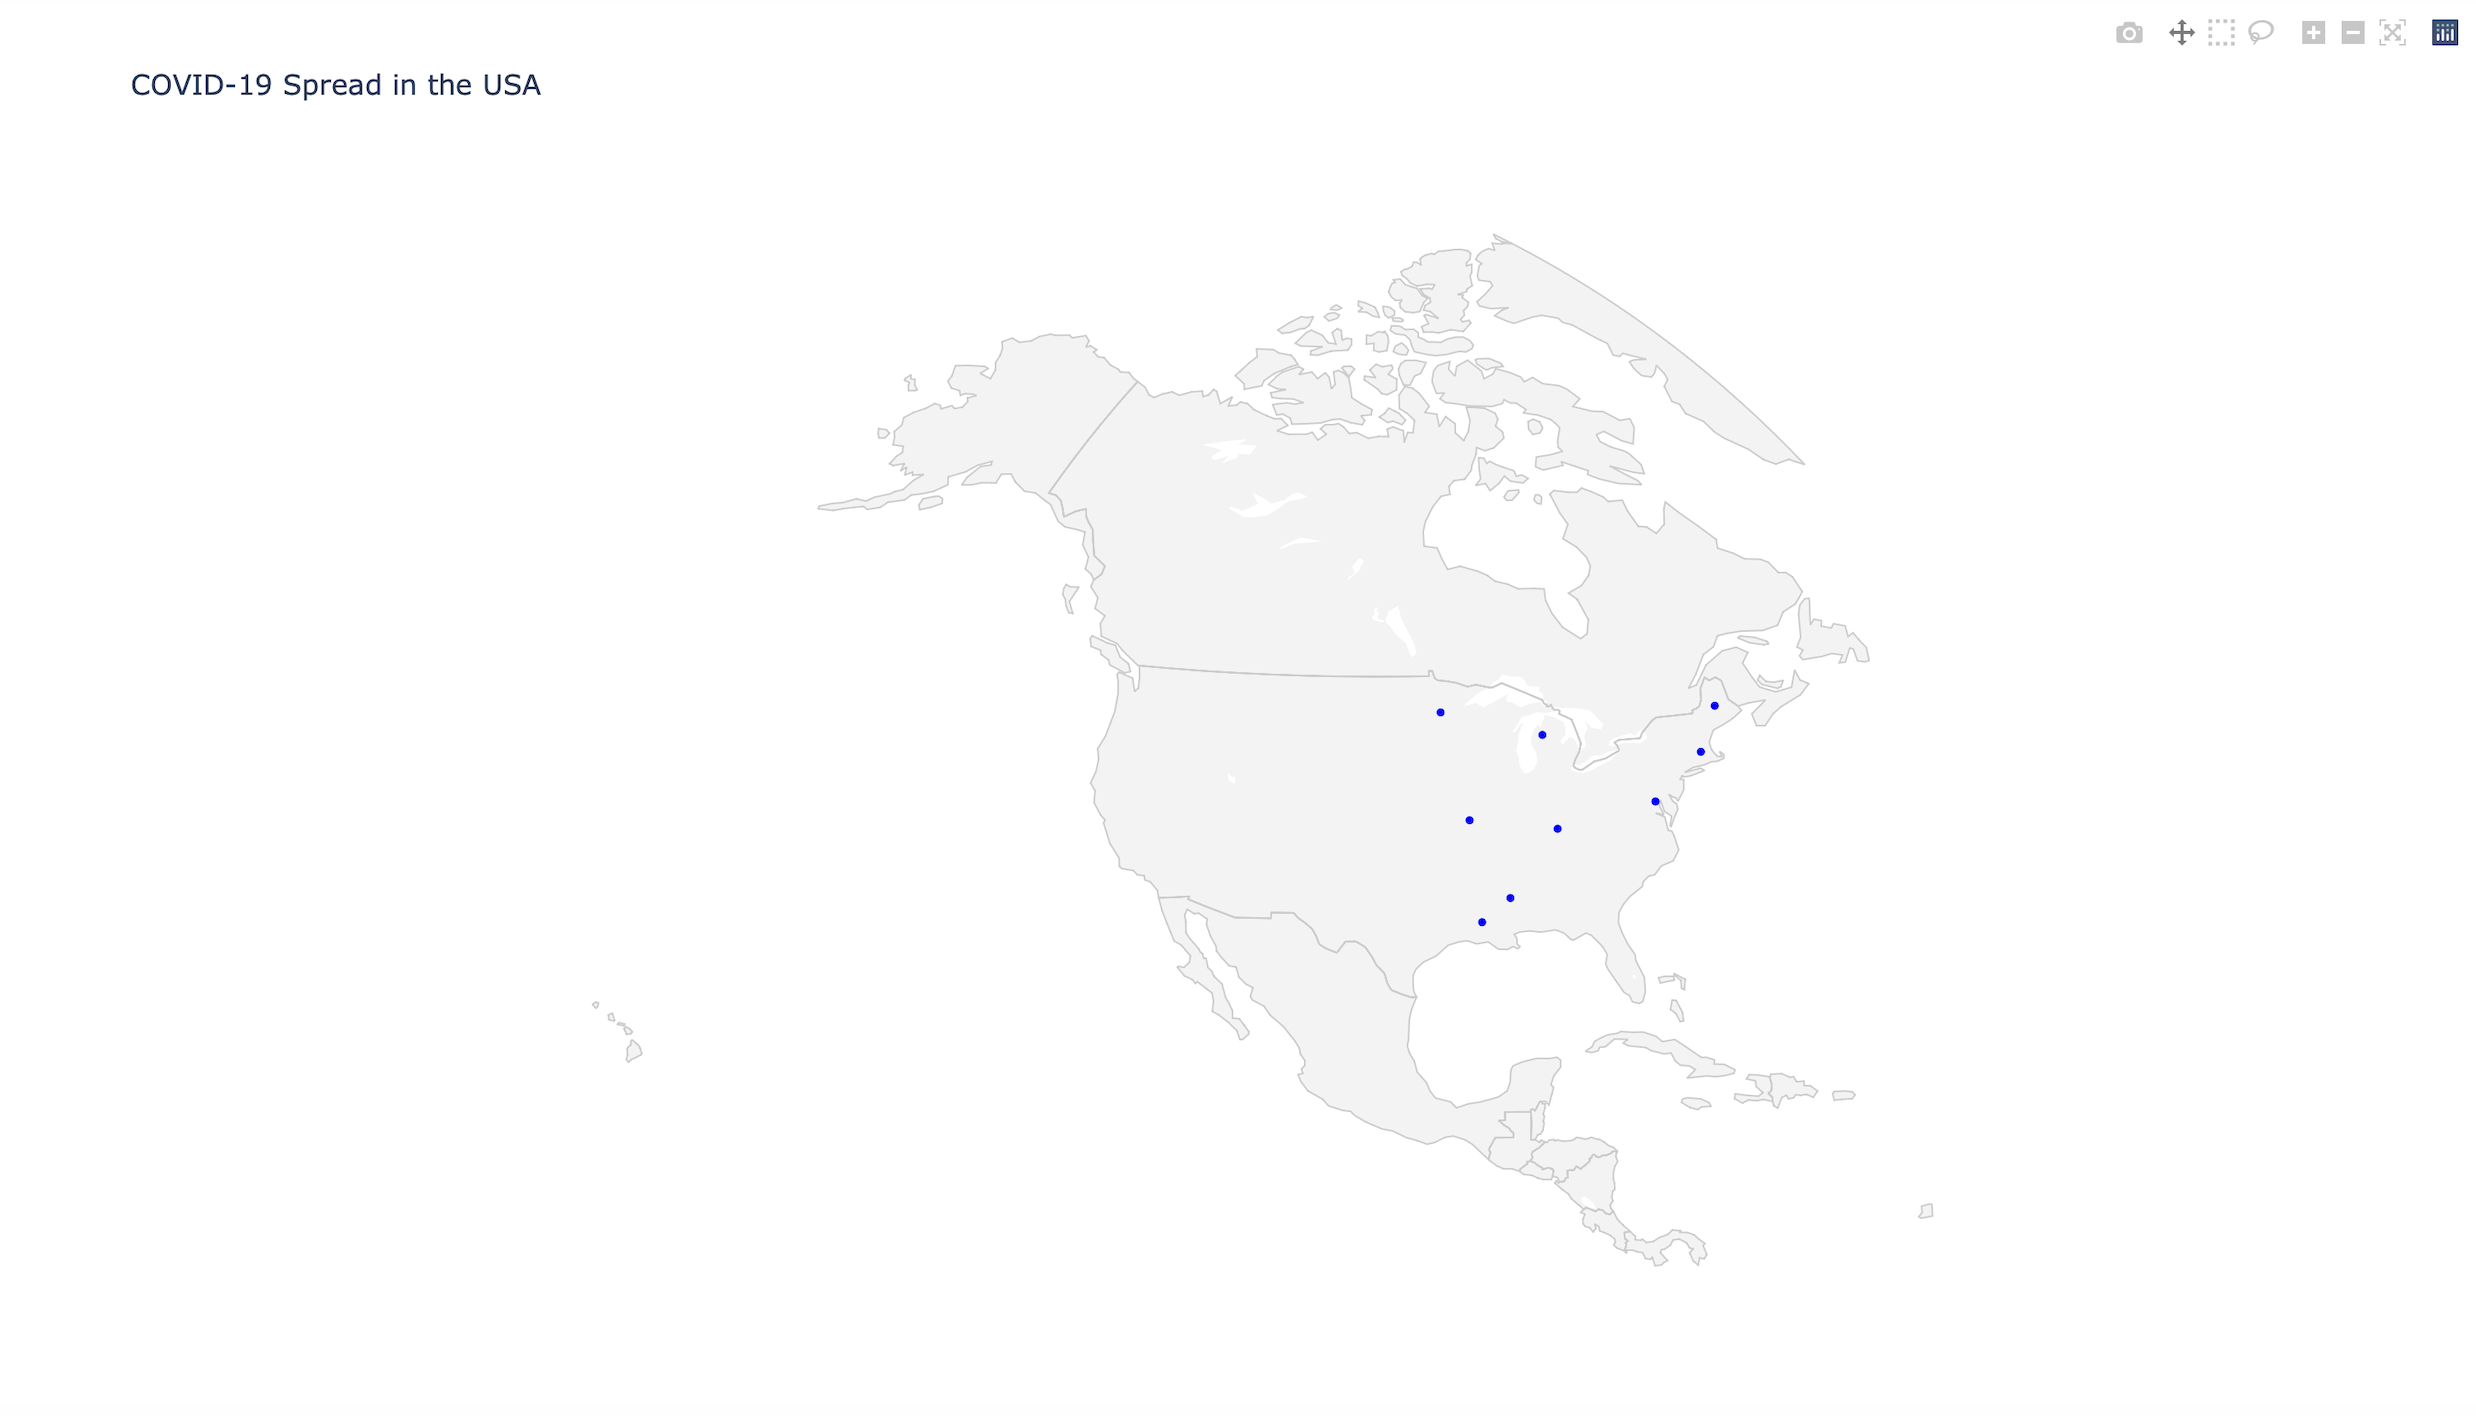
\includegraphics[scale=0.3]{image5.png}

\newpage
\section{Changes to your project plan}
Optimizing and constantly adapting to new timelines, we made some changes to our implementation of this simulation, and the final outcome deviated slightly.\\\\
First of all, we did more research on how disease spreads. Thus we came across the SIR and learned that the $R_0$ approach we intended to use is a subset knowledge of the SIR model. Thus we based our spreading algorithm on the new math.\\\\
Secondly, as we tried to implement the timeline feature of the simulation; however, we found the action of one state infecting multiple states and all these states undergoing the infection in parallel couldn't proceed without using thread parallelism. Although we tried to learn, we realized we had spent too much time getting bogged down by such a time-consuming feature and chose to drop that feature.\\\\
Due to the pressing deadline, we quit making the state select feature where you could hover your cursor to get the infected cases of each state. We changed our plan of having a window-based UI to allow human input to a console-based UI.
Since our algorithm was already complex and we applied what we newly learned from research such as the SIR algorithm and the things we were taught in class such as recursion in infection\_process(), we didn't make query features for the statistics.\\\\
As we ran low on time from all the debugging, we deviated the result from seeing different accumulated cases in each state for making comparisons to displaying the different patterns of the graph structure of infection due to the parameters given in the input.

\newpage
\section{Discussion}
Our original question was how various parameters such as isolation strictness, lockdown policies, vaccination rates, and mask-wearing mandates are effective in controlling the spread of COVID-19. Our question is answered by the fact that different sets of levels of policies produce different degrees of spreading across the country observable from the infected zone patterns.\\\\
The major difficulty that slowed us down was trying to figure out how to put every state's behaviours in sync. We realized it's the idea of thread parallelism that's the key to solving the issue. Tons of time was invested in researching and debugging, in the end, we chose to cancel the implementation because if we had continued down that path, we wouldn't have made a complete program as we do now.\\\\
Aside from the biggest issue, we learned that the question isn't as simple as we thought it was. First, the data we found for the population was from 2018 which could be deprecated to fit under the context of COVID-19.\\\\
Second, we observed that SIR doesn't model and account for all situations absolutely. This is the process of an epidemic that depends on multiple variances.\\\\
Most prominently, the weather and climate of the different seasons play a crucial role. When it's fall, along with flu season, COVID tends to pose a more severe threat. Furthermore, different locations and their population density should also differ in the behaviour of the spread. For instance, the state of California contains a higher population density than Alaska. People in California would have a higher chance of interacting or making contact with people they are surrounded with. Whereas people from Alaska are limited in movement due to the terrain and weather in the area, and there is less population. As our scope of interest is solely on the US, we soon realize the neighbouring countries could also play a role. Most obviously, the major landmass of the US mainland depends on Canada to be connected to Alaska.\\\\
As well as the health properties of each individual, everyone reacts differently to newly existing diseases. The Elderly can experience more severe symptoms, and people with immune deficiency are almost as vulnerable, while others only claim their experience is mild. All of which contribute to the nature of the spread significantly. In our simulation, we made the assumption that each infected person undergoes full recovery after 14 days, yet this is not quite realistic. Some may be able to recover in under a week, while others might try to fight the disease for months.\\\\
The last two ideas come back to make us think about our simulation. In our program, we assumed the rate of contact and removal as some particular values for the people of the whole state. After all, the conditions for the rate of transmission and recovery vary from person to person. Thus that's the limitation for inferring the true behaviour of the pandemic.\\\\
Therefore, although we faced challenges to implement the program and convey the most realistic situation as possible, we still manage to and take pride in being able to create a system that produces the result we intended to find.\\\\
In conclusion, the project was a great exercise for designing, implementing, debugging, and dealing with stress. Since this is the first major project we've done, we learned that we would want to underestimate our capacities in order to build up from the foundations that we're most certain and concrete on.\\\\
Otherwise, we would find ourselves spending hours researching and debugging; as a result, the timeline gets pushed, then some interesting features we have had envisioned to implement won't be possible. The most precious takeaway is that we learned to bypass time-consuming obstacles to not let our grand scheme be affected.

\newpage
\section{References}
$\newline$
Gill, Kieran. “State Populations.” Gist, 12 Nov. 2020, https://gist.github.com/kierangilliam/f80bda\\\n 279998d0485a55f5e4f0ccaf40.\\\\
Interactive Web-Based Data Visualization with R, Plotly, and Shiny, 19 Dec. 2019, \\ \n https://plotly-r.com\\\\
Musa, Salihu S, et al. “Estimation of Exponential Growth Rate and Basic Reproduction\\ \n Number of the Coronavirus Disease 2019 (COVID-19) in Africa - Infectious Diseases of Poverty.” \\ \n Estimation of Exponential Growth Rate and Basic Reproduction Number of the Coronavirus\\ \n Disease 2019 (COVID-19) in Africa, BioMed Central, 16 July 2020, https://idpjournal.biomed- \\\n central.com/articles/10.1186/s40249-020-00718-y. Sievert, Carson. \\\\
Rocks, Tom, director. Oxford Mathematician Explains SIR Disease Model for COVID-19 \\\n (Coronavirus). YouTube, YouTube, 18 Mar. 2020, https://www.youtube.com/watch?v=\\\n NKMHhm2Zbkw. Accessed 27 Mar. 2023. \\\\
Rozanec, Matias. “Distance between Geographic Centers of All US States.” Github, 26 Jan. \n 2022, https://gist.github.com/rozanecm/29926a7c81\\\n 32a0a25e3b12a24abdff86.\\\\
Siff, Andrew, and Myles Miller. “NYC's Unvaccinated Workforce Faces Feb. 11 Termination \n without Proof of Shots.” NYC's Unvaccinated Workforce Faces Feb. 11 Termination Without \n Proof of Shots, NBC New York, 31 Jan. 2022, https://web.archive.org/web/20220201032948/\\ \n https://www.nbcnewyork.com/news/coronavirus/termination-date-set-for-unvaccinated-nypd-officers-\n union/3524922/. \\\\
Smith, David, and Lang Moore. “The Sir Model for Spread of Disease - the Differential Equation \n Model.” The SIR Model for Spread of Disease - The Differential Equation Model, \\\n Mathematical Association of America, Dec. 2004, https://www.maa.org/press/periodicals/loci/joma/\\\n the-sir-model-for-spread-of-disease-the-differential-equation-model. \\\\
Srk. “Covid-19 in USA.” Kaggle, 7 Dec. 2020, https://www.kaggle.com/datasets/sudalairajkumar/covid19- \n in-usa. \\\\
Wells, Chad R, et al. “Impact of International Travel and Border Control Measures on ... - \n Pnas.” Impact of International Travel and Border Control Measures on the Global Spread of \n the Novel 2019 Coronavirus Outbreak, Yoav Keynan, 27 Feb. 2020, https://www.pnas.org/doi/ \n 10.1073/pnas.2002616117.\\\\

\end{document}
